% This is not necessarily in the format for a VUW thesis chapter.

\documentclass[a4paper]{report}

\usepackage{amssymb, amsmath}
\usepackage{tikz}
\usetikzlibrary{calc}

\usepackage{marvosym}


\title{Chapter 4: Effective Slip Length Expressions: Prior Work}
\author{Nat Lund}

\newcommand{\beff}{\ensuremath{b_{\mathrm{eff}}}}
\newcommand{\bhigh}{\ensuremath{b_{\mathrm{high}}}}
\newcommand{\blow}{\ensuremath{b_{\mathrm{low}}}}
\newcommand{\phislip}{\ensuremath{\phi_{\mathrm{slip}}}}
\newcommand{\phisol}{\ensuremath{\phi_{\mathrm{solid}}}}
\newcommand{\sigsol}{\ensuremath{\sigma_{\mathrm{solid}}}}
\newcommand{\gamsol}{\ensuremath{ \dot{\gamma}_{\mathrm{solid}} }} 

\newcommand{\sep}{\begin{equation*} \star \end{equation*}}

%\vspace{1em}
%\colorbox[gray]{0.8}{ \textsc{Other Results} }
%\vspace{0.5em}

\newcommand{\paper}[1]
         {\colorbox[gray]{0.8}{ \textsc{#1}}
         
         }

\begin{document}
\maketitle

This thesis presents a new expression for the effective slip length of mixed-slip surfaces.  To establish the novelty, we must place our new expression in the context of other results in this field.  Hence, this chapter is a literature review of the field of effective slip.  The results of this thesis are already published as three papers in this field; thus, the work of this thesis is easily placed in context amongst other peer-reviewed papers.

There are a small number of results for effective slip lengths in the literature.  In this chapter, we survey a dozen or so of them.  This cannot pretend to be comprehensive --- there may be results hidden in obscure journals, behind paywalls, or camouflaged by nonstandard terminology.  Further, mathematically equivalent results may exist in fields unrelated to fluid mechanics.  There is nothing we can do about this.  The best we can claim to do is present some `high profile' results in the field of fluid slip.

\subsection*{Categorizing Results by Regime of Applicability}

The published results for an effective slip length are applicable in different physical situations.  It is useful to sort these different regimes by the following criteria:

\begin{itemize}

\item \textbf{Navier Stokes} versus \textbf{Stokes}.  A few results use the full Navier Stokes description of fluid flow.  However, slip is very small scale phenomenon, so the characteristic length scale of the flow is also very small.  Thus, the Reynolds number is very small, and the Navier Stokes equation is very well approximated by the simpler Stokes flow equation.  (This is covered fully in the next chapter.)  Accordingly, most results have been derived assuming only Stokes `creeping' flow.

\item \textbf{Flat} versus \textbf{Rough}. Assuming the boundary to be the flat plane $z=0$ is a major simplification, warranted on grounds of mathematical tractability.  Two thirds of effective slip results make this assumption.

\item \textbf{2-D Flow} (1-D Surface) versus \textbf{3-D Flow} (2-D Surface).
If the surface is symmetric in one dimension, then the flow above it will have the same symmetry.  Thus, full three-dimensional flow reduces to two-dimensional flow over a one-dimensional surface pattern.  About half of effective slip results tackle this simpler case.

\item \textbf{Perfect-slip/Zero-slip Binary Surface} or \textbf{Not.}  Assuming a binary surface, comprising regions of either vanishing slip ($b=0$), or perfect slip ($b \rightarrow \infty$) only, can enable considerable simplification of the mathematics.  Half of all effective slip results tackle this limiting case.

\end{itemize}

These categories are used to construct Table \ref{table:slipresults}.  All the papers that we shall survey in this section appear in the table, in their appropriate categories.  Some papers appear in more than one cell; in that case, the paper presents more than one result.  Note that if a paper gives a \emph{single} result for a case that \emph{subsumes} another case (eg. a 3-D result that is automatically valid for the 2-D case), then the paper appears in only \emph{one} cell.


\begin{table}
\caption{The papers (presenting effective slip lengths) surveyed in this section, 
categorized into their applicable regimes.}
\label{table:slipresults}

\begin{center}
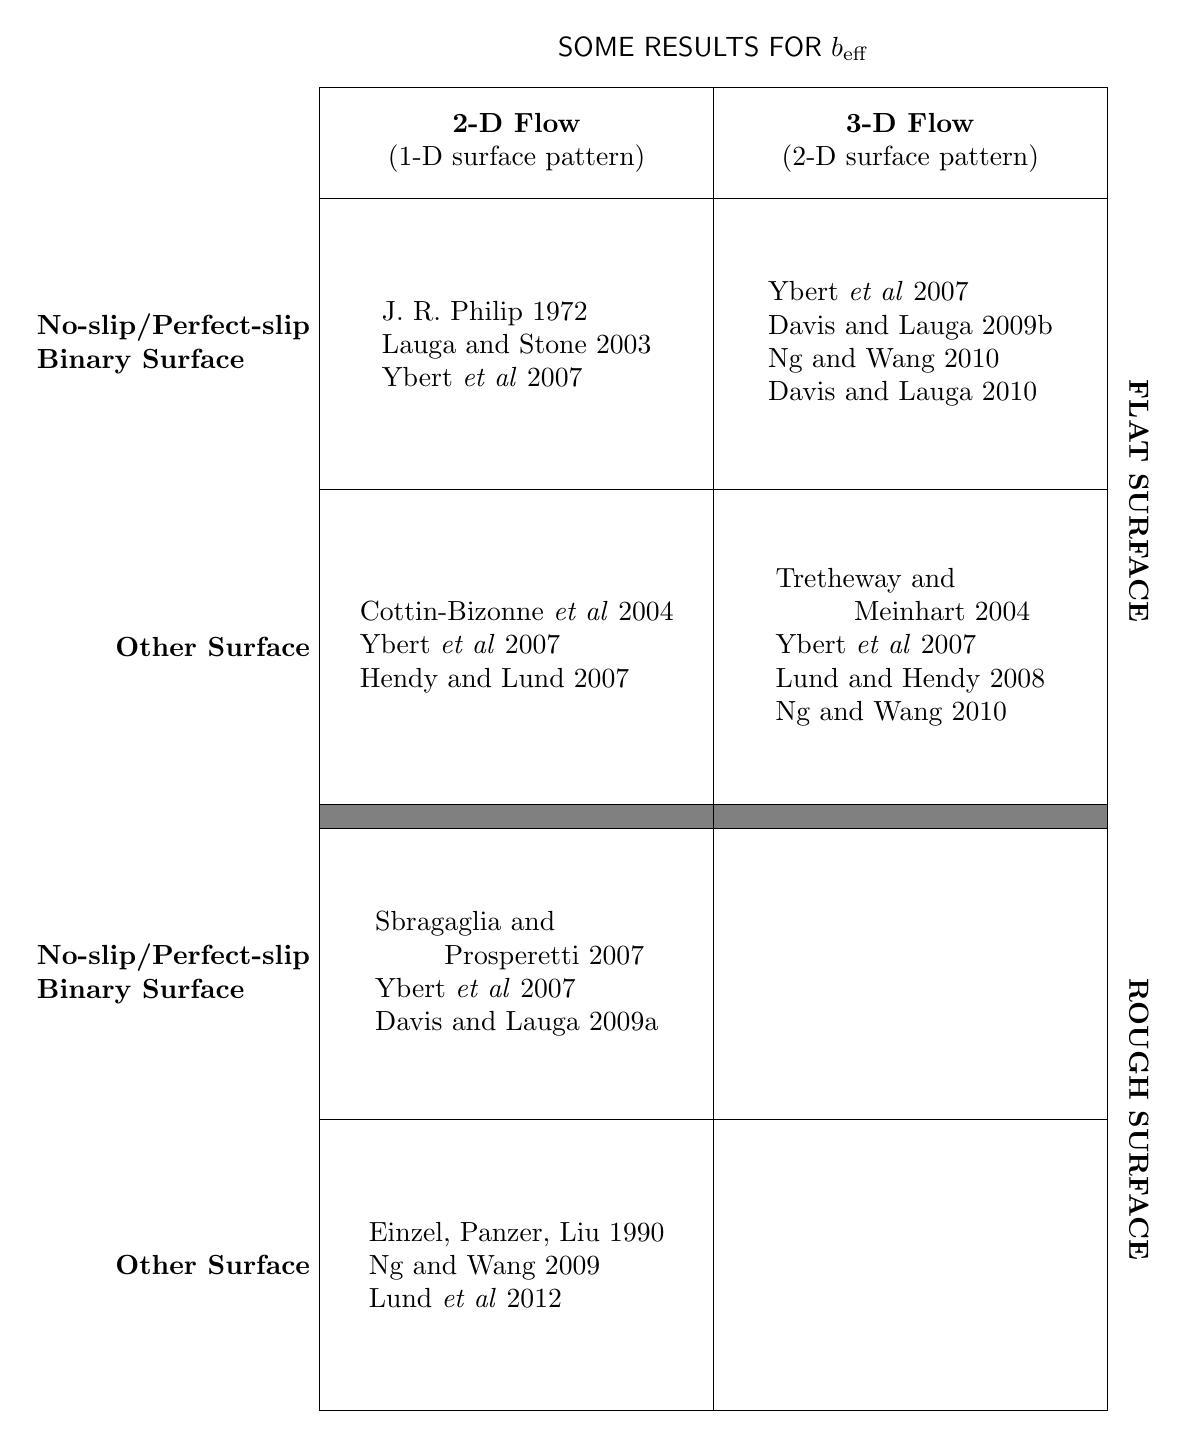
\begin{tikzpicture}

% Manually define half width of table.
\path (5,0) coordinate (midway);

% Manually define row heights.
\path (0,3.7) coordinate (flatbinary);
\path (0,4) coordinate (flatother);
\path (0,3.7) coordinate (roughbinary);
\path (0,3.7) coordinate (roughother);

\path (0,0.3) coordinate (sepwidth);

\path (0,1.4) coordinate (labelbox);

%%%%%%%%%%%%%%%%%%%%%%%%%%%%%%%%%%%%%%%%% Tikz calculates all other points...
% Bottom left corner is origin (0,0)
\path (0,0) ++(midway) coordinate (midbottom);

\path (0,0) ++(roughother) coordinate (lowdiv);
\path (lowdiv) ++(roughbinary) coordinate (belowsep);
\path (belowsep) ++(sepwidth) coordinate (abovesep);
\path (abovesep) ++(flatother) coordinate (highdiv);
\path (highdiv) ++(flatbinary) coordinate (celltop);
\path (celltop) ++ (labelbox) ++(midway) coordinate (topmid);
\path (topmid) ++(midway) coordinate (topright);


%%%%%%%%%%%%%%%%%%%%%%%%%%%%%%%%%%%%%%% Draw all boxes and lines...
\draw (0,0) rectangle (topright);
\draw (celltop) -- ++(midway) -- ++(midway);
\draw (highdiv) -- ++(midway) -- ++(midway);
\draw [fill=gray] (abovesep) ++(midway) ++(midway) rectangle (belowsep);
\draw (lowdiv) -- ++(midway) -- ++(midway);
\draw (topmid) -- (midbottom);

%%%%%%%%%%%%%%%%%%%%%%%%%%%%%%%%%%%%%%% Add flow type labels.
\path (celltop) --         coordinate[midway] (2Dlabel) (topmid);
\path (2Dlabel) ++(midway) coordinate (3Dlabel);
\node at (2Dlabel)[align=center] {\textbf{2-D Flow}\\(1-D surface pattern)};
\node at (3Dlabel)[align=center] {\textbf{3-D Flow}\\(2-D surface pattern)};

%%%%%%%%%%%%%%%%%%%%%%%%%%%%%%%%%%%%%%   Labels for surface types
\path (abovesep) -- coordinate[midway] (midflat) (celltop);
\path (0,0) --      coordinate[midway] (midrough) (belowsep);
\path (midflat) ++(midway) ++(midway) ++(0.4,0) coordinate (flatlabel);
\path (midrough) ++(midway) ++(midway) ++(0.4,0) coordinate (roughlabel);
\node at (flatlabel)  [rotate=270] {\textbf{FLAT SURFACE}};
\node at (roughlabel) [rotate=270] {\textbf{ROUGH SURFACE}};

%%%%%%%%%%%%%%%%%%%%%%%%%%%%%%%%%%%%%%%%%%%%%%%%%%%  Points in middle of rows...
\path (celltop)  -- coordinate[midway] (row1) (highdiv);
\path (highdiv)  -- coordinate[midway] (row2) (abovesep);
\path (belowsep) -- coordinate[midway] (row3) (lowdiv);
\path (lowdiv)   -- coordinate[midway] (row4) (0,0);

%%%%%%%%%%%%%%%%%%%%%%%%%%%%%%%%%%%%%%%%%%%%%%  Labels for Binary or Other surface types.
\node at (row1) [left, align=left] {\textbf{No-slip/Perfect-slip}\\
										\textbf{Binary Surface}};
\node at (row2) [left, align=left] {\textbf{Other Surface}};
\node at (row3) [left, align=left] {\textbf{No-slip/Perfect-slip}\\
										\textbf{Binary Surface}};
\node at (row4) [left, align=left] {\textbf{Other Surface}};

%%%%%%%%%%%%%%%%%%%%%%%%%%%%%%%%%%%%%%%%%%%%%%%%%  Locations of Text nodes...
%%%%%%%%%%%%  2-D Flow
\path (row1) -- coordinate[midway] (flatbin2D) +(midway);
\path (row2) -- coordinate[midway] (flatother2D) +(midway);
\path (row3) -- coordinate[midway] (roughbin2D) +(midway);
\path (row4) -- coordinate[midway] (roughother2D) +(midway);
%%%%%%%%%%%%%%  3-D Flow
\path (flatbin2D) ++(midway) coordinate (flatbin3D);
\path (flatother2D) ++(midway) coordinate (flatother3D);
\path (roughbin2D) ++(midway) coordinate (roughbin3D);
\path (roughother2D) ++(midway) coordinate (roughother3D);

%%%%%%%%%%%%%%%%%%%%%%%%%%%%%%%%%%%%%%%%%%%%%   LABEL FOR WHOLE TABLE
\path (topmid) ++(0,0.5) coordinate (heading);
\node at (heading) {\textsf{SOME RESULTS FOR \beff} };


%%%%%%%%%%%%%%%%%%%%%%%%%%%%%%%%%%%%%%%%%%%%%%%  Contents of Cells.....

\node at (flatbin2D) [align=left]
							{
							J. R. Philip 1972 \\
							Lauga and Stone 2003 \\
							Ybert \emph{et al} 2007
							};
							
\node at (flatbin3D) [align=left]
							{
							Ybert \emph{et al} 2007 \\
							Davis and Lauga 2009b \\
							Ng and Wang 2010 \\
							Davis and Lauga 2010
							};
							
\node at (flatother2D) [align=left]
							{
							Cottin-Bizonne \emph{et al} 2004 \\
							Ybert \emph{et al} 2007 \\
							Hendy and Lund 2007
							};
							
\node at (flatother3D) [align=left]
							{
							Tretheway and \\
								\phantom{mmm} Meinhart 2004 \\
							Ybert \emph{et al} 2007 \\
							Lund and Hendy 2008 \\
							Ng and Wang 2010
							};
							
\node at (roughbin2D) [align=left]
							{
							Sbragaglia and \\
								\phantom{mmm}Prosperetti 2007 \\
							Ybert \emph{et al} 2007 \\
							Davis and Lauga 2009a
							};

\node at (roughbin3D) [align=left]
							{
							
							};
							
\node at (roughother2D) [align=left]
							{
							Einzel, Panzer, Liu 1990 \\
							Ng and Wang 2009 \\
							Lund \emph{et al} 2012
							};

\node at (roughother3D) [align=left]
							{
							
							};
							
\end{tikzpicture}
\end{center}

\end{table}

\newpage


\subsection*{Categorizing Results by Mathematical Strength}

As well as sorting the published $\beff$ results by the regime of applicability, we can sort them by the rigour of their derivation.

Mathematicians may describe a result as `exact'.  This usually means that it is in a form that can be written down as an explicit formula.  The benefit of an exact result is practical: it can be evaluated more easily.  Whether a result is exact or not is nothing to do with the rigour of its derivation; i.e. unrelated to the \emph{strength} of the result. 

In mathematics, a result is described as \emph{strong} if \emph{few assumptions} were made in its derivation.  The fewer the assumptions, the `stronger' the result.
There are two benefits of a strong result: First, because it relies on fewer assumptions, it is likely to be more widely applicable.  So `strong' means `more general'.  Secondly, the fewer assumptions, the fewer modes of failure.  Assumptions some times turn out to be false; this sad event may cause various results to be overturned.  A strong result is more robust.  It is less fragile to nasty surprises as the body of human knowledge grows.  (Note that a strong result may have a long complicated derivation, and thus be vulnerable to errors in the derivation.  The point is that a stronger result has a more \emph{self contained} derivation.)

Obviously, in theoretical physics we would like our results to be as useful and trustworthy as possible --- `exact' and `strong'.  For the purposes of this literature review, we shall rank the published results using the following (somewhat arbitrary) labels.

\begin{itemize}

\item \textbf{Derived} Results.  A relation for $\beff$ derived (mathematically) from the Stokes equation, an appropriate boundary condition, and perhaps an assumption of fluid incompressibility.

\end{itemize}

Other results:

\begin{itemize}

\item \textbf{Scaling Law} Results.  May or may not include more assumptions than a Derived Result, but the result is not exact, giving $\beff$ only as a multiple of some other length scale.

\item \textbf{Simplified} Results.  Further simplifying assumptions have been made, from reasonable phenomenological models to mere hand waving.

\item \textbf{Empirical} Results.  Exact results that express a curve fitted to either numerical or experimental data.  May be informed by stronger results.

\end{itemize}


There are comparatively fewer Derived Results.  They are listed in Table \ref{table:derivedslip}.  The other results are listed in Table \ref{table:otherslip}.

\begin{table}
\caption{The papers surveyed here in which $\beff$ is rigorously derived from only the Stokes equation, an appropriate boundary condition and perhaps the assumption of fluid incompressibility.}
\label{table:derivedslip}

\begin{center}
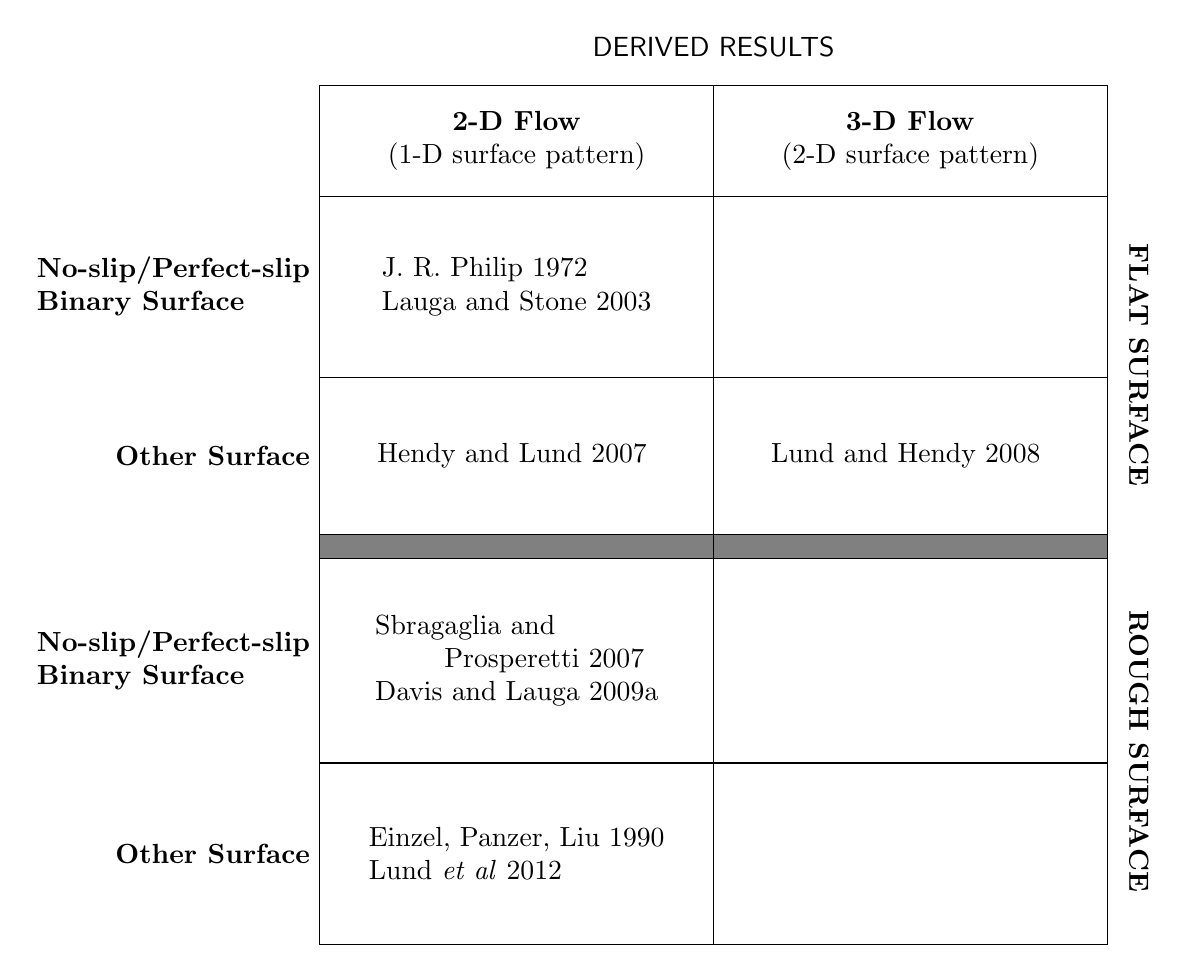
\begin{tikzpicture}

% Manually define half width of table.
\path (5,0) coordinate (midway);

% Manually define row heights.
\path (0,2.3) coordinate (flatbinary);
\path (0,2) coordinate (flatother);
\path (0,2.6) coordinate (roughbinary);
\path (0,2.3) coordinate (roughother);

\path (0,0.3) coordinate (sepwidth);

\path (0,1.4) coordinate (labelbox);

%%%%%%%%%%%%%%%%%%%%%%%%%%%%%%%%%%%%%%%%% Tikz calculates all other points...
% Bottom left corner is origin (0,0)
\path (0,0) ++(midway) coordinate (midbottom);

\path (0,0) ++(roughother) coordinate (lowdiv);
\path (lowdiv) ++(roughbinary) coordinate (belowsep);
\path (belowsep) ++(sepwidth) coordinate (abovesep);
\path (abovesep) ++(flatother) coordinate (highdiv);
\path (highdiv) ++(flatbinary) coordinate (celltop);
\path (celltop) ++ (labelbox) ++(midway) coordinate (topmid);
\path (topmid) ++(midway) coordinate (topright);


%%%%%%%%%%%%%%%%%%%%%%%%%%%%%%%%%%%%%%% Draw all boxes and lines...
\draw (0,0) rectangle (topright);
\draw (celltop) -- ++(midway) -- ++(midway);
\draw (highdiv) -- ++(midway) -- ++(midway);
\draw [fill=gray] (abovesep) ++(midway) ++(midway) rectangle (belowsep);
\draw (lowdiv) -- ++(midway) -- ++(midway);
\draw (topmid) -- (midbottom);

%%%%%%%%%%%%%%%%%%%%%%%%%%%%%%%%%%%%%%% Add flow type labels.
\path (celltop) --         coordinate[midway] (2Dlabel) (topmid);
\path (2Dlabel) ++(midway) coordinate (3Dlabel);
\node at (2Dlabel)[align=center] {\textbf{2-D Flow}\\(1-D surface pattern)};
\node at (3Dlabel)[align=center] {\textbf{3-D Flow}\\(2-D surface pattern)};

%%%%%%%%%%%%%%%%%%%%%%%%%%%%%%%%%%%%%%   Labels for surface types
\path (abovesep) -- coordinate[midway] (midflat) (celltop);
\path (0,0) --      coordinate[midway] (midrough) (belowsep);
\path (midflat) ++(midway) ++(midway) ++(0.4,0) coordinate (flatlabel);
\path (midrough) ++(midway) ++(midway) ++(0.4,0) coordinate (roughlabel);
\node at (flatlabel)  [rotate=270] {\textbf{FLAT SURFACE}};
\node at (roughlabel) [rotate=270] {\textbf{ROUGH SURFACE}};

%%%%%%%%%%%%%%%%%%%%%%%%%%%%%%%%%%%%%%%%%%%%%%%%%%%  Points in middle of rows...
\path (celltop)  -- coordinate[midway] (row1) (highdiv);
\path (highdiv)  -- coordinate[midway] (row2) (abovesep);
\path (belowsep) -- coordinate[midway] (row3) (lowdiv);
\path (lowdiv)   -- coordinate[midway] (row4) (0,0);

%%%%%%%%%%%%%%%%%%%%%%%%%%%%%%%%%%%%%%%%%%%%%%  Labels for Binary or Other surface types.
\node at (row1) [left, align=left] {\textbf{No-slip/Perfect-slip}\\
										\textbf{Binary Surface}};
\node at (row2) [left, align=left] {\textbf{Other Surface}};
\node at (row3) [left, align=left] {\textbf{No-slip/Perfect-slip}\\
										\textbf{Binary Surface}};
\node at (row4) [left, align=left] {\textbf{Other Surface}};

%%%%%%%%%%%%%%%%%%%%%%%%%%%%%%%%%%%%%%%%%%%%%%%%%  Locations of Text nodes...
%%%%%%%%%%%%  2-D Flow
\path (row1) -- coordinate[midway] (flatbin2D) +(midway);
\path (row2) -- coordinate[midway] (flatother2D) +(midway);
\path (row3) -- coordinate[midway] (roughbin2D) +(midway);
\path (row4) -- coordinate[midway] (roughother2D) +(midway);
%%%%%%%%%%%%%%  3-D Flow
\path (flatbin2D) ++(midway) coordinate (flatbin3D);
\path (flatother2D) ++(midway) coordinate (flatother3D);
\path (roughbin2D) ++(midway) coordinate (roughbin3D);
\path (roughother2D) ++(midway) coordinate (roughother3D);

%%%%%%%%%%%%%%%%%%%%%%%%%%%%%%%%%%%%%%%%%%%%%   LABEL FOR WHOLE TABLE
\path (topmid) ++(0,0.5) coordinate (heading);
\node at (heading) {\textsf{DERIVED RESULTS} };


%%%%%%%%%%%%%%%%%%%%%%%%%%%%%%%%%%%%%%%%%%%%%%%  Contents of Cells.....

\node at (flatbin2D) [align=left]
							{
							J. R. Philip 1972 \\
							Lauga and Stone 2003
							};
							
\node at (flatbin3D) [align=left]
							{
							};
							
\node at (flatother2D) [align=left]
							{
							Hendy and Lund 2007
							};
							
\node at (flatother3D) [align=left]
							{
							Lund and Hendy 2008
							};
							
\node at (roughbin2D) [align=left]
							{
							Sbragaglia and \\
								\phantom{mmm}Prosperetti 2007 \\
							Davis and Lauga 2009a
							};

\node at (roughbin3D) [align=left]
							{
							
							};
							
\node at (roughother2D) [align=left]
							{
							Einzel, Panzer, Liu 1990 \\
							Lund \emph{et al} 2012
							};

\node at (roughother3D) [align=left]
							{
							
							};
							
\end{tikzpicture}
\end{center}

\end{table}


%\vspace*{2em}

\begin{table}
\caption{The papers surveyed here in which $\beff$ is not exact, or does not have a rigorous derivation.}
\label{table:otherslip}

\begin{center}
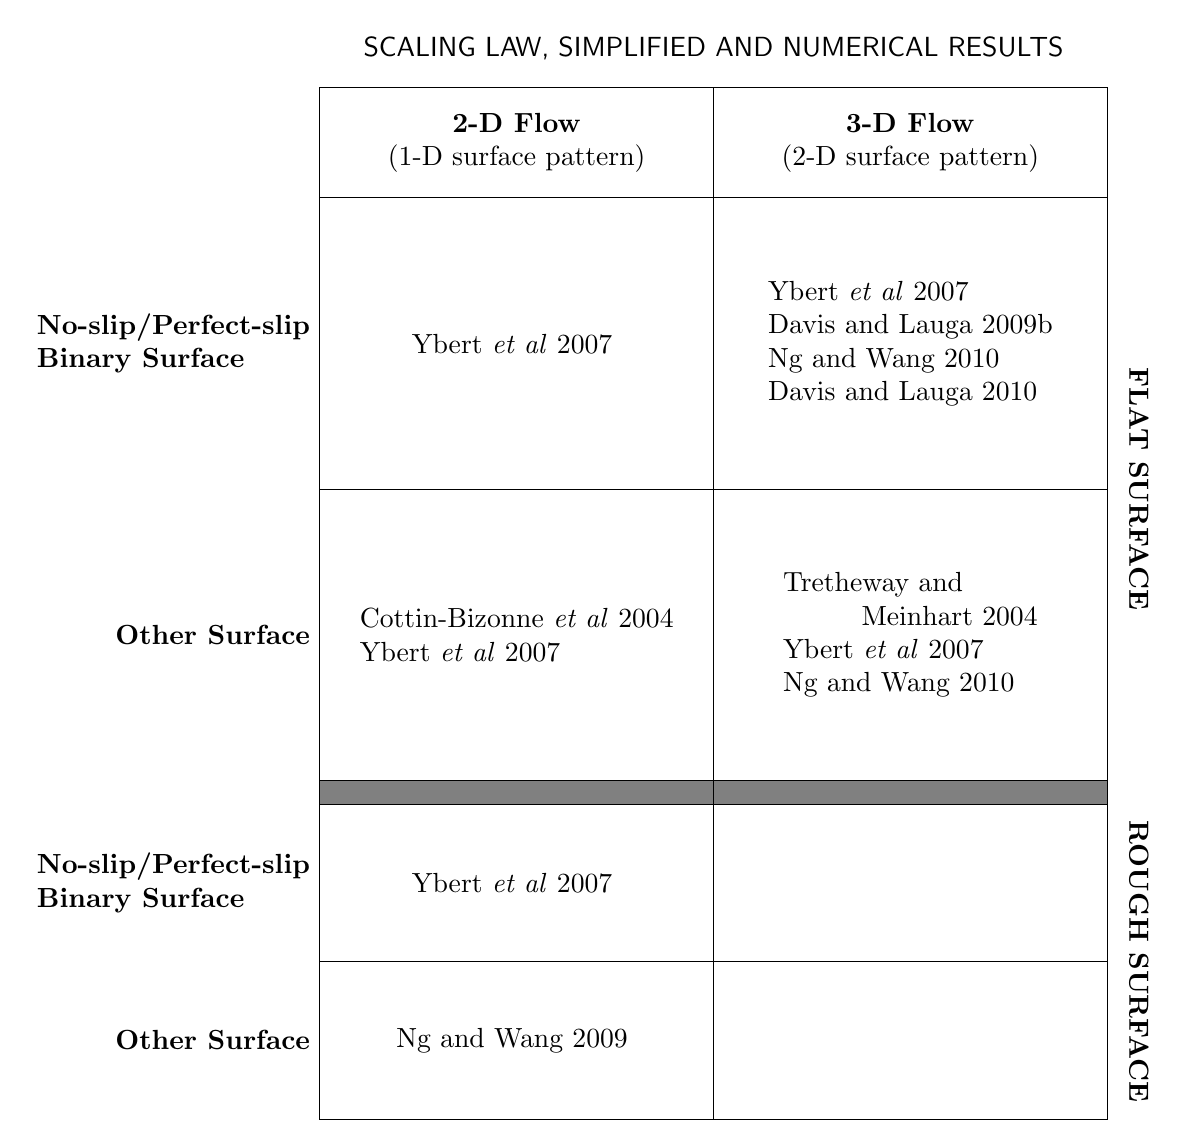
\begin{tikzpicture}

% Manually define half width of table.
\path (5,0) coordinate (midway);

% Manually define row heights.
\path (0,3.7) coordinate (flatbinary);
\path (0,3.7) coordinate (flatother);
\path (0,2) coordinate (roughbinary);
\path (0,2) coordinate (roughother);

\path (0,0.3) coordinate (sepwidth);

\path (0,1.4) coordinate (labelbox);

%%%%%%%%%%%%%%%%%%%%%%%%%%%%%%%%%%%%%%%%% Tikz calculates all other points...
% Bottom left corner is origin (0,0)
\path (0,0) ++(midway) coordinate (midbottom);

\path (0,0) ++(roughother) coordinate (lowdiv);
\path (lowdiv) ++(roughbinary) coordinate (belowsep);
\path (belowsep) ++(sepwidth) coordinate (abovesep);
\path (abovesep) ++(flatother) coordinate (highdiv);
\path (highdiv) ++(flatbinary) coordinate (celltop);
\path (celltop) ++ (labelbox) ++(midway) coordinate (topmid);
\path (topmid) ++(midway) coordinate (topright);


%%%%%%%%%%%%%%%%%%%%%%%%%%%%%%%%%%%%%%% Draw all boxes and lines...
\draw (0,0) rectangle (topright);
\draw (celltop) -- ++(midway) -- ++(midway);
\draw (highdiv) -- ++(midway) -- ++(midway);
\draw [fill=gray] (abovesep) ++(midway) ++(midway) rectangle (belowsep);
\draw (lowdiv) -- ++(midway) -- ++(midway);
\draw (topmid) -- (midbottom);

%%%%%%%%%%%%%%%%%%%%%%%%%%%%%%%%%%%%%%% Add flow type labels.
\path (celltop) --         coordinate[midway] (2Dlabel) (topmid);
\path (2Dlabel) ++(midway) coordinate (3Dlabel);
\node at (2Dlabel)[align=center] {\textbf{2-D Flow}\\(1-D surface pattern)};
\node at (3Dlabel)[align=center] {\textbf{3-D Flow}\\(2-D surface pattern)};

%%%%%%%%%%%%%%%%%%%%%%%%%%%%%%%%%%%%%%   Labels for surface types
\path (abovesep) -- coordinate[midway] (midflat) (celltop);
\path (0,0) --      coordinate[midway] (midrough) (belowsep);
\path (midflat) ++(midway) ++(midway) ++(0.4,0) coordinate (flatlabel);
\path (midrough) ++(midway) ++(midway) ++(0.4,0) coordinate (roughlabel);
\node at (flatlabel)  [rotate=270] {\textbf{FLAT SURFACE}};
\node at (roughlabel) [rotate=270] {\textbf{ROUGH SURFACE}};

%%%%%%%%%%%%%%%%%%%%%%%%%%%%%%%%%%%%%%%%%%%%%%%%%%%  Points in middle of rows...
\path (celltop)  -- coordinate[midway] (row1) (highdiv);
\path (highdiv)  -- coordinate[midway] (row2) (abovesep);
\path (belowsep) -- coordinate[midway] (row3) (lowdiv);
\path (lowdiv)   -- coordinate[midway] (row4) (0,0);

%%%%%%%%%%%%%%%%%%%%%%%%%%%%%%%%%%%%%%%%%%%%%%  Labels for Binary or Other surface types.
\node at (row1) [left, align=left] {\textbf{No-slip/Perfect-slip}\\
										\textbf{Binary Surface}};
\node at (row2) [left, align=left] {\textbf{Other Surface}};
\node at (row3) [left, align=left] {\textbf{No-slip/Perfect-slip}\\
										\textbf{Binary Surface}};
\node at (row4) [left, align=left] {\textbf{Other Surface}};

%%%%%%%%%%%%%%%%%%%%%%%%%%%%%%%%%%%%%%%%%%%%%%%%%  Locations of Text nodes...
%%%%%%%%%%%%  2-D Flow
\path (row1) -- coordinate[midway] (flatbin2D) +(midway);
\path (row2) -- coordinate[midway] (flatother2D) +(midway);
\path (row3) -- coordinate[midway] (roughbin2D) +(midway);
\path (row4) -- coordinate[midway] (roughother2D) +(midway);
%%%%%%%%%%%%%%  3-D Flow
\path (flatbin2D) ++(midway) coordinate (flatbin3D);
\path (flatother2D) ++(midway) coordinate (flatother3D);
\path (roughbin2D) ++(midway) coordinate (roughbin3D);
\path (roughother2D) ++(midway) coordinate (roughother3D);

%%%%%%%%%%%%%%%%%%%%%%%%%%%%%%%%%%%%%%%%%%%%%   LABEL FOR WHOLE TABLE
\path (topmid) ++(0,0.5) coordinate (heading);
\node at (heading) {\textsf{SCALING LAW, SIMPLIFIED AND NUMERICAL RESULTS} };


%%%%%%%%%%%%%%%%%%%%%%%%%%%%%%%%%%%%%%%%%%%%%%%  Contents of Cells.....

\node at (flatbin2D) [align=left]
							{
							Ybert \emph{et al} 2007
							};
							
\node at (flatbin3D) [align=left]
							{
							Ybert \emph{et al} 2007 \\
							Davis and Lauga 2009b \\
							Ng and Wang 2010 \\
							Davis and Lauga 2010
							};
							
\node at (flatother2D) [align=left]
							{
							Cottin-Bizonne \emph{et al} 2004 \\
							Ybert \emph{et al} 2007
							
							};
							
\node at (flatother3D) [align=left]
							{
							Tretheway and \\
								\phantom{mmm} Meinhart 2004 \\
							Ybert \emph{et al} 2007 \\
							Ng and Wang 2010
							};
							
\node at (roughbin2D) [align=left]
							{
							Ybert \emph{et al} 2007
							};

\node at (roughbin3D) [align=left]
							{
							
							};
							
\node at (roughother2D) [align=left]
							{
							Ng and Wang 2009
							};

\node at (roughother3D) [align=left]
							{
							};
							
\end{tikzpicture}
\end{center}

\end{table}


\vspace{2em}

\clearpage

\section*{Derived Results}

All results are for 2-dimensional flow (over a 1-dimensional surface pattern), unless otherwise noted.

\subsection*{Flat Surface, of No-Slip and Perfect-Slip Parallel Strips}

\paper{J.\ R.\ Philip 1972}
The paper that arguably started it all is J.\ R.\ Philip's article in ZAMP in 1972 \cite{Philip1972}.  This comprehensive effort studied amongst other things ``Shear Flow over a Plate with a Regular Array of Longitudinal No-Shear Slots".  Philip uses the phrase `no-shear' to mean what we might now call `perfect-slip'.  The no-shear slots are parallel to the direction of flow.   He generalizes a device by Karush and Young, a conformal mapping in the complex plane, to prove that in the far field:

\[ \beff= \frac{L}{\pi}	\ln \sec \frac{\pi}{2} \phislip \]

where $L$ is the period of the array, and $\phislip$ is the fraction of the surface that has perfect slip. This proof is replicated in Appendix B. 

\begin{center}
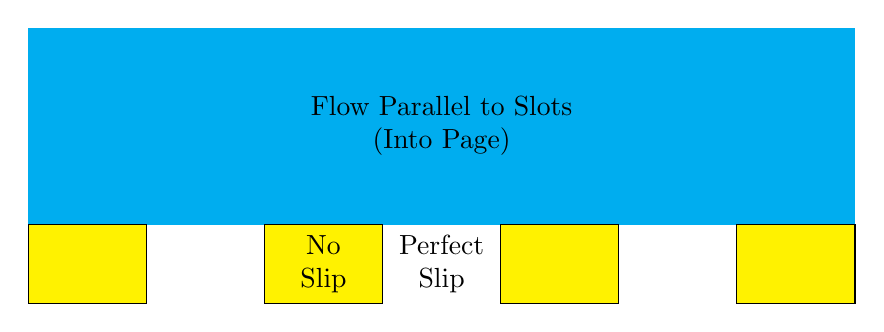
\begin{tikzpicture}

\coordinate (slotwidth) at +(1.5,0);
\coordinate (topright) at ($7*(slotwidth) + (0,2.5)$);
\fill[cyan] (0,0) rectangle (topright);

\path (slotwidth) ++(0,-1) coordinate (box);

\foreach \n in {0,1,2,3}
    \draw[fill=yellow] ($2*\n*(slotwidth)$) rectangle +(box);

\path ($2*(slotwidth) $) -- node[align=center] {No\\ Slip} +(box);
\path ($3*(slotwidth) $) -- node[align=center] {Perfect\\ Slip} +(box);

\path (0,0) -- node[align=center] {Flow Parallel to Slots\\ (Into Page)} (topright);

\end{tikzpicture}
\end{center}
The above schematic shows the no-slip/perfect-slip longitudinal flow system studied by J.\ R.\ Philip.

\sep

\paper{Lauga \& Stone 2003}
It wasn't until 2003 that the case for flow \emph{transverse} to the slots was solved.  
In an article in the Journal of Fluid Mechanics that year \cite{LaugaStone2003}, Lauga and Stone study pressure-driven Stokes flow down a straight circular pipe.  They note that there is no analytic solution for the transverse case.  They derive dual series of equations, one for each boundary slip, which are simultaneously true.  They solve these numerically.  With $\phislip$ fixed, the asymptotic limit of the numerical solutions as period $L \rightarrow 0$ is the far field flow, implying an effective slip length:

\[ \beff= \frac{1}{2} \frac{L}{\pi}	\ln \sec \frac{\pi}{2} \phislip \]

which is exactly half the solution for parallel slots.

They provide a physical interpretation for the factor of two: An elongated body falling under its own weight falls twice as fast if it is oriented vertically than if it is oriented horizontally.

\begin{center}
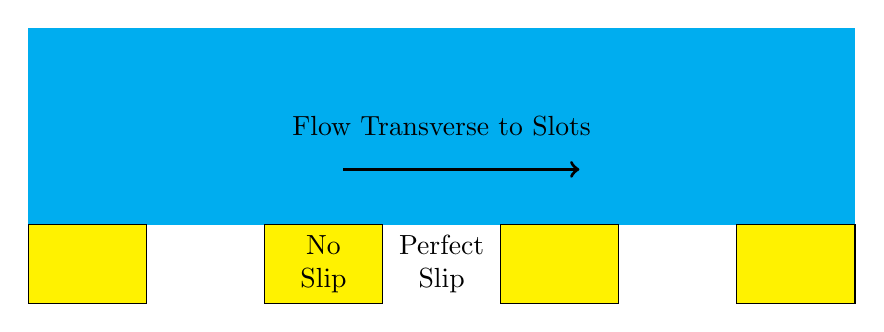
\begin{tikzpicture}

\coordinate (slotwidth) at +(1.5,0);
\coordinate (topright) at ($7*(slotwidth) + (0,2.5)$);
\fill[cyan] (0,0) rectangle (topright);

\path (slotwidth) ++(0,-1) coordinate (box);

\foreach \n in {0,1,2,3}
    \draw[fill=yellow] ($2*\n*(slotwidth)$) rectangle +(box);

\path ($2*(slotwidth) $) -- node[align=center] {No\\ Slip} +(box);
\path ($3*(slotwidth) $) -- node[align=center] {Perfect\\ Slip} +(box);

\path (0,0) -- node[align=center] {Flow Transverse to Slots} (topright);
\draw[->,very thick] (4,0.7) -- +(3,0);

\end{tikzpicture}
\end{center}

The schematic above depicts the no-slip/perfect-slip transverse flow system studied by Lauga \& Stone.


\subsection*{Flat No-Slip and Curved Perfect-Slip Parallel Strips}

\paper{Sbragaglia \& Prosperetti 2007}
Philip's foundational solution had flat strips of perfect slip.  Since these model a stress-free liquid-gas interface, it is reasonable to extend the model so that the perfect slip surface forms a slightly curved meniscus.  In 2007, Sbragaglia and Prosperetti did exactly that \cite{SbragagliaProsperetti2007}.  Using a dual-series technique, (rather than conformal mapping), they replicate Philip's result, and add a perturbation due the the curved meniscus.  They use as a small perturbation parameter:

\[ \epsilon = \frac{1}{2\pi} \frac{L}{2R} \]

where $R$ is the radius of curvature, and $L$ is the period of the pattern.  In the far field, the effective slip length is:

\[ \beff= \frac{L}{\pi}	\ln \sec \frac{\pi}{2} \phislip - \frac{L^2}{4R}\phislip^3 \int_0^1 
\frac{[1-\cos(\pi\phislip s)] (1-s^2) }{\cos(\pi\phislip s) - \cos(\pi\phislip)}
\; ds \]

They note that deformation of the meniscus \emph{reduces} the slip length. ``The physical origin of this phenomenon is due to the fact that, when the interface bows into the groove, the condition of free shear (perfect slip) is moved below the level $z=0$ of the undisturbed surface so that, on $z=0$, there is a residual nonzero stress."

\begin{center}
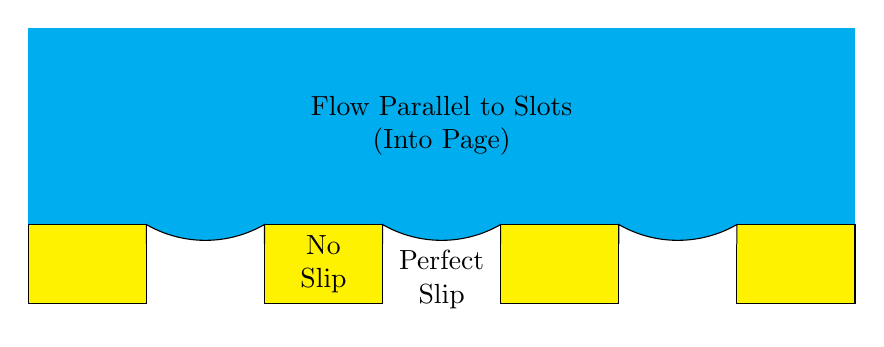
\begin{tikzpicture}

\coordinate (slotwidth) at +(1.5,0);
\coordinate (topright) at ($7*(slotwidth) + (0,2.5)$);
\fill[cyan] (0,-0.23) rectangle (topright);

\path (slotwidth) ++(0,-1) coordinate (box);

\foreach \n in {0,1,2,3}
    \draw[fill=yellow] ($2*\n*(slotwidth)$) rectangle +(box);

\path ($2*(slotwidth) $) -- node[align=center] {No\\ Slip} +(box);
\path ($3*(slotwidth) + (0,-0.2)$) -- node[align=center] {Perfect\\ Slip} +(box);

\path (0,0) -- node[align=center] {Flow Parallel to Slots\\ (Into Page)} (topright);

%\foreach \n in {1,3,5}
%    \draw[fill=cyan] ($\n*(slotwidth)$) arc (240:300:1.5);
    
\foreach \n in {1,3,5}
\draw[fill=white] ($\n*(slotwidth) + (0,-0.25) $) -- ++(0,0.25) arc (240:300:1.5) -- +(0,-0.25);

\end{tikzpicture}
\end{center}

\sep

\paper{Davis \& Lauga 2009a}
Another variation is that the perfect-slip strips model a bubble type geometry, with the surface bulging up into the liquid.  In a 2009 paper in Physics of Fluids, Davis and Lauga consider this scenario \cite{DavisLauga2009a}.  Their model is still 2-dimensional Stokes flow, so that the `bubbles' can be considered to be the cross sections of spherical caps on top of channels full of air. Flow is thus transverse to the grating.  The channels have width $2c$, and the greater the air pressure therein, the further the bubble cap protrudes into the liquid.  The magnitude of protrusion is quantified by the angle $\theta$ that the bubble wall makes to the solid surface.

In the dilute limit, i.e. bubbles sparsely distributed on the surface, the effective slip tends to:

\begin{multline*}
\beff = c\pi \phislip \; \times \\
\int_0^{\infty}
\frac{s}{\sinh 2s(\pi -  \theta) + s \sin 2\theta}  \left[ \cos 2\theta + 
\frac{s \sin 2\theta \cosh s \pi + \sinh s(\pi - 2 \theta)}{\sinh s \pi}
\right] \; ds
\end{multline*}

\vspace{1em}

\begin{center}
\begin{tikzpicture}

\coordinate (width) at (10.5,0);
\fill[cyan] (0,2.5) rectangle (width);

\coordinate (b1) at (1.5,0);
\draw[fill=white] ($(b1) + (0,-1.5)$) -- ++(0,1.5) arc (145:35:1.07) -- +(0,-1.5) coordinate (p1);
\path (b1) -- node[above, align=center] {Perfect\\Slip} (p1);

\coordinate (b2) at (8,0);
\draw[fill=white] ($(b2) + (0,-1.5)$) -- ++(0,1.5) arc (145:35:1.07) -- +(0,-1.5) coordinate (p2);
\draw[<->] (b2) ++(0,-1) -- node[above] {$2c$} ($(p2) +(0,0.5)$);
\draw[dashed] (b2) -- +(0.8,0) (b2) -- +(55:1 cm);
\path (b2) ++(0.4,0.15) node {$\theta$};


\draw[fill=yellow] (0,0) ++(0,-1.5) rectangle (b1);
\draw[fill=yellow] (p1) rectangle (b2);
\draw[fill=yellow] (p2) rectangle (width);

\node at (5,0) [below] {No Slip};

\path (0,0) -- node[align=center] {Flow Transverse to Slots} (topright);
\draw[->,very thick] (4,0.7) -- +(3,0);

\end{tikzpicture}
\end{center}

They evaluate for various values of $\theta$, nondimensionalized by channel width.  They find good agreement with the numerical results of Steinberger \emph{et al} \cite{Steinberger2007} and Hyv\"{a}luoma and Harting \cite{HyvaluomaHarting2008}.

``The main features of the full numerical results are seen to be reproduced by our analytical model.  There exists a critical protrusion angle $ \theta_c$ above which the effect of the wall-attached bubbles displays a transition from reduced ($ \theta < \theta_c $) to enhanced friction ($ \theta > \theta_c $).  Our model predicts $ \theta \approx 65^{\circ} $, in good agreement with the results of [Steinberger \emph{et al}] ($ \theta \approx 62^{\circ} $) and [Hyv\"{a}luoma and Harting] ($ \theta \approx 69^{\circ} $). ''

\subsection*{Flat Surface, with Slip Length $\gg$ Period, Otherwise Arbitrary}

\paper{Hendy \& Lund 2007}
In 2007, we published in Phys. Rev. E \cite{HendyLund2007} a perturbative proof that --- to first order --- the effective slip length is the harmonic mean of the intrinsic slip lengths

\begin{equation*}
\beff = \left< \frac{1}{b} \right>^{-1}
\end{equation*}

This result is valid for a flat surface with an intrinsic slip length varying in one dimension over some period $L$.  The minimum slip length must be greater than the period $L$, but may otherwise be arbitrary.

\vspace{1em}
\colorbox[gray]{0.8}{ \textsc{3-D Flow} }
\vspace{0.5em} \\

\paper{Lund \& Hendy 2008}
In 2008, we published in ANZIAM Journal \cite{LundHendy2008} an extension of the above result for 3-dimensional flow over a flat surface with a square-periodic variation in intrinsic slip length.  The perturbative proof still required that $b_{\mathrm{minimum}} \gg L$, with $b$ otherwise arbitrary, and the result was the same harmonic mean formula:

\begin{equation*}
\beff = \left< \frac{1}{b} \right>^{-1}
\end{equation*}

This published result subsumes our published result from the previous year.  It is is fully presented in Chapter 7.

\subsection*{Rough Surface, with Slip Length $\gg$ Period, Otherwise Arbitrary}

\paper{Lund \emph{et al} 2012}
Using a completely different technique --- homogenization --- we have proved that
for flow over a \emph{rough} surface with a slip length varying with the same period $L$ as the roughness, with the minimum slip length much greater than $L$,

\begin{equation*}
\beff = \left< \frac{\sqrt{1 + s^2}}{b} \right>^{-1}
\end{equation*}

This is the harmonic mean weighted by \emph{area of contact} --- not just footprint area.  ($s$ is the slope and $\sqrt{1+s^2}$ is the arc length.)  For a flat surface, this reduces to our previous perturbative result.

This proof was published in Phys. Rev. E in 2012 \cite{Lund2012}.  It is the centrepiece of this thesis, and is presented fully in Chapter 6.


\subsection*{Rough Surface of Single Intrinsic Slip}

\paper{Einzel, Panzer \& Liu 1990}
Finally, there is an interesting relatively early result for a \emph{rough} surface with a \emph{single} unchanging intrinsic slip length.  In 1990 Einzel, Panzer and Liu \cite{EinzelPanzerLiu1990} studied a `weakly varying surface' of the form

\begin{equation*}
y(x) = \sum_n \left[ h_n^{\cos} \cos(nkx) + h_n^{\sin} \sin(nkx) \right]
\end{equation*} 

This Fourier surface has a \textbf{single} intrinsic slip length $b_0$.  In the `stick' limit, $kb_0 \ll 1$, the effective slip length is:

\begin{equation*}
\beff = b_0 - \sum_n nk \left[ (h_n^{\cos})^2 + (h_n^{\sin})^2  \right]
\end{equation*}

More interestingly, in the limit of perfect slip, $kb_0 \gg 1$, they get

\begin{equation*}
\beff = \left[ \frac{1}{b_0} + \sum_n (nk)^3 \left[ (h_n^{\cos})^2 + (h_n^{\sin})^2 \right]
 \right]^{-1}
\end{equation*}

They get a very similar result for incommensurate sine waves, so the result holds for pseudo-random roughness.

The interesting point is that even if a rough surface has \emph{perfect slip} i.e. infinite slip length, the effective slip length is still finite, because of the roughness.


\section*{Simplified Models, Scaling Laws and Numerics}

\subsection*{Models with Simplifying Assumptions}

\paper{Tretheway \& Meinhart 2004}
In 2004, Tretheway and Meinhart \cite{TrethewayMeinhart2004} consider a variation of the binary surface wherein the gas-liquid interface has some large finite slip length, rather than an infinite slip length.  Piecing together the paper and an Erratum \cite{TrethewayMeinhartErratum2004} published 2 years later, it seems they claim that the intrinsic slip length for water of thickness $2D$ flowing over a rarefied gas layer of thickness $\delta$ is:

\begin{equation*}
b_{\mathrm{slip}} = \frac{1}{2D} \left( \frac{\mu_{water}}{\mu_{air}} \right)
\left[ 2D\delta + \delta^2 + \epsilon(4D + 2\delta) \right]
\end{equation*}

where $\epsilon$ is the slip length of the rarefied gas slipping over the solid.  $b_{\mathrm{slip}}$ is derived from a velocity equation $u_{\mathrm{slip}}$.  They combine this with the standard no-slip velocity equation (Couette flow):
``We combine the slip and no-slip [velocity] equations in a weighted average and calculate the cumulative velocity, $u_{\mathrm{cu.}}$, by

\begin{equation*}
u_{\mathrm{cu.}} = \phi u_{\mathrm{slip}} + (1-\phi) u_{\mathrm{no-slip}}
\end{equation*}

where $\phi$ is the fraction covered by gas. ..., we set the cumulative velocity at the air-water interface equal to the slip length times the shear rate at the air-water interface to obtain an equation for slip length ..."

\begin{equation*}
b_{\mathrm{cu.}} = \phi \frac{1}{2D} \left( \frac{\mu_{water}}{\mu_{air}} \right)
 \left[ 2D\delta + \delta^2 + \epsilon(4D + 2\delta) \right]
\end{equation*}

And that is the end of their analysis.  However, the observant reader may notice that

\begin{equation*}
b_{\mathrm{cu.}} = \phi b_{\mathrm{slip}} 
\end{equation*}

Perhaps due to the inconsistent notation of a derivation spread over a paper and an erratum published two years later, Tretheway and Meinhart do not mention this.

Furthermore, a careful reading seems to reveal that 
$ \partial_z u_{\mathrm{slip}} = \partial_z u_{\mathrm{no-slip}} = \dot{\gamma} $
If the shear rate does not depend on the local slip length, we can think about a binary surface with more general slip conditions --- not just `no slip', with local slip lengths defined via
$u_{\mathrm{slip}} = b_{\mathrm{slip}} \dot{\gamma}$ and $u_{\mathrm{low-slip}} = b_{\mathrm{low-slip}} \dot{\gamma}$.

Then for velocities at the $z=0$ boundary:
\begin{align*}
u_{\mathrm{cu.}} & = b_{\mathrm{cu.}} \partial_z u_{\mathrm{cu.}} \\
u_{\mathrm{cu.}} & = b_{\mathrm{cu.}} \partial_z
[ \phi u_{\mathrm{slip}} + (1-\phi) u_{\mathrm{low-slip}} ] \\
u_{\mathrm{cu.}} & = b_{\mathrm{cu.}} 
[ \phi \partial_z u_{\mathrm{slip}} + (1-\phi) \partial_z u_{\mathrm{low-slip}} ] \\
u_{\mathrm{cu.}} & = b_{\mathrm{cu.}} [ \phi \dot{\gamma} + (1-\phi) \dot{\gamma} ]\\
u_{\mathrm{cu.}} & = b_{\mathrm{cu.}} \dot{\gamma}\\
\phi u_{\mathrm{slip}} + (1-\phi) u_{\mathrm{low-slip}} & = b_{\mathrm{cu.}} \dot{\gamma} \\
\phi \frac{u_{\mathrm{slip}}}{\dot{\gamma}} + (1-\phi) \frac{ u_{\mathrm{low-slip}}} {\dot{\gamma}} & = b_{\mathrm{cu.}} \\
\phi b_{\mathrm{slip}} + (1-\phi) b_{\mathrm{low-slip}} & = b_{\mathrm{cu.}} \\
\left< b \right> & = b_{\mathrm{cu.}}
\end{align*}

Thus, their definition of `cumulative velocity' appears to imply that $b_{\mathrm{cu.}}$ is simply the area-weighted average of local slip lengths.  If $b_{\mathrm{low-slip}} = 0$, it follows that 
$ b_{\mathrm{cu.}} = \phi b_{\mathrm{slip}} $.

\sep

\paper{Cottin-Bizonne \emph{et al} 2004}
A rather more convincing assumption was used in a landmark article in Eur. Phys. Journal E in 2004 by Cecile Cottin-Bizonne \emph{et al} \cite{Cottin-Bizonne2004}.

Cottin-Bizonne and colleagues presented molecular dynamics fluid simulations, in which they observed the `dewetting transition', wherein the liquid sits on top of posts, giving a large effective slip length.  They do some numerical calculations to predict the effective slip length in various regimes.  

For the regime of \textbf{No-slip/Perfect-slip} strips, they find excellent agreement with the analytic results of J.\ R.\ Philip \cite{Philip1972} and Lauga and Stone \cite{LaugaStone2003}.  Now confident in their technique, they investigate other regimes.

For strips of \textbf{No-slip and Partial-slip} material, they find that $\beff$ is fixed by the smaller of the two lengths, $b_{\mathrm{slip}}$ and the period $L$.

$\bullet$ For low slip ($b_{\mathrm{slip}} < L$), $\beff$ increases linearly, roughly $\beff = b_{\mathrm{slip}} / 4$

$\bullet$ For high slip ( $b_{\mathrm{slip}} > 10L$), $\beff$ asymptotes to a fraction of $L$. Roughly $L/10$ for flow parallel to stripes, and $L/20$ for transverse flow.

\vspace{1em}

For stripes of \textbf{Partial-slip and Perfect-slip} material, they find that $\beff$ is determined by the \emph{larger} of $b_{\mathrm{slip}}$ and period $L$.

$\bullet$ For small slip ($b_{\mathrm{slip}} \ll L$), $\beff$ is fixed by the period $L$.

$\bullet$ For high slip ($b_{\mathrm{slip}} > L$), $\beff$ increases linearly with intrinsic slip.

They advance a `simple phenomenological model' to explain this linearity:

``We introduce the interfacial friction coefficient $\lambda$, defined by ... the continuity of the tangential stress $\sigma_s$ at the solid-liquid interface:
\begin{equation*}
\sigma_s = \eta \frac{\partial V}{\partial z} = \lambda V_s
\end{equation*}
where $\eta$ is the viscosity of the liquid and $V_s$ [is the slip velocity]. The interfacial friction coefficient $\lambda$ is then related to the slip length $b$ by
\begin{equation*}
\lambda = \frac{\eta}{b}
\end{equation*}
The effective friction coefficient $\Lambda = \frac{\eta}{\beff}$ can be interpreted as the \emph{averaged friction} over the different stripes, and we obtain, accordingly, the following result for the effective macroscopic slip length as a function of the microscopic ones:
\begin{equation*}
\beff = \left[ \phi \frac{1}{ b_{\mathrm{high}} }  + (1 -\phi) \frac{1}{ b_{\mathrm{low}}} \right]^{-1}
\end{equation*}
which is similar to the addition rule for resistors in parallel.

In the case $b_{\mathrm{high}} \rightarrow \infty$, we expect
\begin{equation*}
\beff = \frac{b_{\mathrm{low}}}{1-\phi} \;"
\end{equation*}

Cecile notes ``It is important to emphasize that its validity is limited to the case where both the slip lengths, $\bhigh$ and $\blow$, are larger than the roughness periodicity $L$. Note, however, that in practice, this relationship is valid down to $\blow > 0.1L$."

To the best of our knowledge, this is the first assertion that $\beff$ is the harmonic mean of intrinsic slip lengths.  This result inspired this thesis, which provides a rigorous derivation and extension of this harmonic mean formula.

\sep

\paper{Ng \& Wang 2009}
In 2009, Ng and Wang \cite{NgWang2009} considered flow over the familiar binary surface of flat perfect-slip/partial-slip regions, with one difference: the perfect-slip gas-liquid interface was allowed to be some distance $d$ below the solid surface.  They did numerical evaluations of flow both parallel and transverse to the resulting `step function profile' surface.

They compare their numerics with the continuum modeling results of Cottin-Bizonne \emph{et al.}\ 2004 \cite{Cottin-Bizonne2004}, and find essentially perfect agreement.

However, their most interesting observation relates to the conventional completely flat binary surface.  They recall Cottin-Bizonne's proposal for $\beff$ for flow parallel to the strips:

\begin{equation*}
\beff = \frac{b_{\mathrm{solid}}}{1 - \phi}
\end{equation*}

which works very well for large $b_{\mathrm{solid}}$.  Ng and Wang have discovered that this is much improved by simply gluing on J.\ Philip's exact result \cite{Philip1972} for $b_{\mathrm{solid}}=0$:

\begin{equation*}
\beff =  \frac{L}{\pi} \ln \left[ \sec \left( \frac{\pi}{2} \phi \right) \right] +
 \frac{b_{\mathrm{solid}}}{1 - \phi}
\end{equation*}

And similarly, for transverse flow, glue on the exact solution of Lauga and Stone \cite{LaugaStone2003}
\begin{equation*}
\beff = \frac{1}{2}  \frac{L}{\pi} \ln \left[ \sec \left( \frac{\pi}{2} \phi \right) \right] +
 \frac{b_{\mathrm{solid}}}{1 - \phi}
\end{equation*}

Ng and Wang test these extended formulae numerically, and find that they give a maximum error of 3\% -- 6\%, compared with Cottin-Bizonne's original formula which can have a maximum error of more than 50\% for small $b_{\mathrm{solid}}$.


\subsection*{The Scaling Laws of Ybert \emph{et al}}

\paper{Ybert \emph{et al} 2007}
Possibly the highest-profile article relating to effective slip length is the 2007 article in Physics of Fluids by Ybert and coworkers, entitled ``Achieving large slip with superhydrophobic surfaces: Scaling laws for generic geometries" \cite{Ybert2007}. The authors form a research group at Lyon, France, which includes Cecile Cottin-Bizonne.  Hence, the paper makes the same assumptions as the `phenomenological model' of Cottin-Bizonne 2004 \cite{Cottin-Bizonne2004}, and takes them in a slightly different direction, to get scaling laws for various geometries.
The paper is sufficiently influential, and the derivation sufficiently elegant, that we essentially reproduce it here.


At the heart of the model is the concept of stress balance.  Consider the stress on a plane of infinitesimal area located on the fluid boundary.

\begin{center}
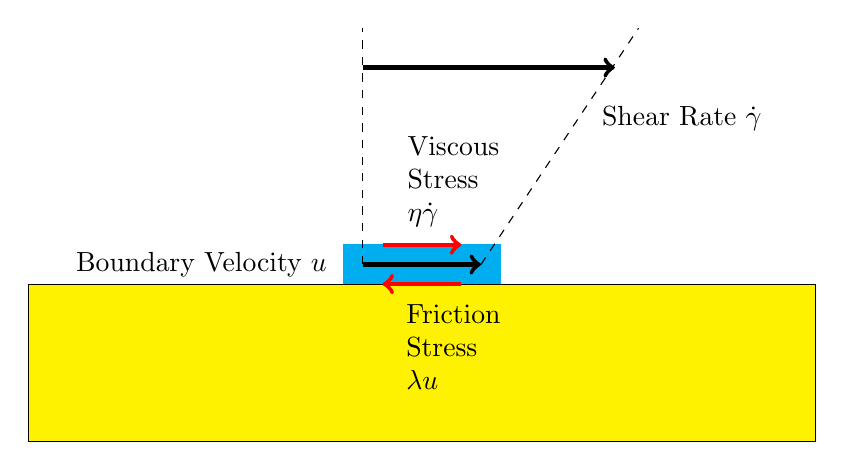
\begin{tikzpicture}

\filldraw[color=cyan] (0,0) rectangle (2,0.5);
\draw [fill=yellow] (-4,0) rectangle (6,-2);

\coordinate (ref) at (0.25,0.25);
\draw[->,ultra thick] (ref) -- ++(1.5,0);
\draw[dashed] (ref) -- ++(0,3);
\draw[->, ultra thick] (ref) ++(0,2.5) -- ++(3.2,0);
\draw[dashed] (ref) ++(1.5,0) -- ++(2,3);

\node at (-1.8,0.25) {Boundary Velocity $u$};
\node at (4.3,2.1) {Shear Rate $\dot{\gamma}$};

%%%%%%%%%%%%%%  Stress arrows
\draw [<-, ultra thick, color=red] (0.5,0) -- ++(1,0);
\draw [->, ultra thick, color=red] (0.5,0.5) -- ++(1,0);

\node at (1.4,1.3) [align=left] {Viscous\\ Stress\\ $\eta \dot{\gamma} $};
\node at (1.4,-0.8) [align=left] {Friction\\Stress\\ $\lambda u$};

\end{tikzpicture}
\end{center}

At equilibrium, the stresses balance:

\begin{equation*}
\sigma = \eta \dot{\gamma} = \lambda u
\end{equation*}

The stress can be \emph{averaged} over the entire surface (or over one period):

\begin{equation*}
\left< \sigma \right> = \left< \eta \dot{\gamma} \right> = \left< \lambda u \right>
\end{equation*}

Now the viscosity $\eta$ can be considered constant throughout the fluid, so that $  \left< \eta \dot{\gamma} \right> = \eta \left< \dot{\gamma} \right> $.  But the friction coefficient $\lambda$ is not constant.  Therefore, Ybert \emph{et al} define an effective friction coefficient such that:

\begin{equation*}
\left< \lambda u \right> = \lambda_{\mathrm{eff}} \left< u \right>
\end{equation*}
\begin{equation*}
\text{But then of course} \quad
\eta \left< \dot{\gamma} \right> = \lambda_{\mathrm{eff}} \left< u \right>
%\end{equation*}
\quad \text{rearranges to}  \quad
%\begin{equation*}
\left< u \right> = \frac{\eta}{ \lambda_{\mathrm{eff}} } \left< \dot{\gamma} \right> 
\end{equation*}
which defines some kind of effective slip length:
\begin{equation*}
\beff = \frac{\eta}{ \lambda_{\mathrm{eff}} }  
\end{equation*}

This definition of $\beff$ relates the \emph{area average} boundary velocity to the \emph{area average} of the shear rate at the boundary.

\begin{equation*}
\left< u \right> = \beff \left< \dot{\gamma} \right> 
\end{equation*}

\vspace*{1em}
\colorbox[gray]{0.8}{ \textsc{2-D Flow over Perfect-slip/No-slip Surface} }
\vspace{0.5em}

The average stress on a binary surface can be decomposed into the area-weighted averages of the `subaverages' of stress over the liquid-gas interface and the liquid-solid interface:

Then 
\begin{equation*}
\left< \sigma \right> = \phi \left< \sigma_{\mathrm{gas}} \right> + 
\phisol \left<  \sigsol \right> 
\end{equation*}

If the gas-liquid interface is considered to be perfect-slip or \emph{no-shear}, there is no stress; $ \sigma_{\mathrm{gas}} = 0 $.  Hence 
\begin{equation*}
\left< \sigma \right> = \phisol \left<  \sigsol \right>
\end{equation*}

\begin{equation*}
\text{Viscosity $\eta$ is constant, so} \;\;\;
\left< \sigsol \right> = \eta \left< \dot{\gamma}_{\mathrm{solid}} \right>
\end{equation*}
\begin{equation*}
\text{For flow over a flat surface, `simple shear' obtains:} \quad
\dot{\gamma}_{\mathrm{solid}} = \frac{\partial u}{\partial z}
\end{equation*}

So
\begin{equation*}
\left< \sigsol \right> = \eta \left< \frac{\partial u}{\partial z} \right>
\end{equation*}

\vspace{1em}
\colorbox[gray]{0.8}{ \textsc{Case where $\phisol \rightarrow 0$, Mostly Plug-like flow.} }
\vspace{0.5em}

\begin{center}
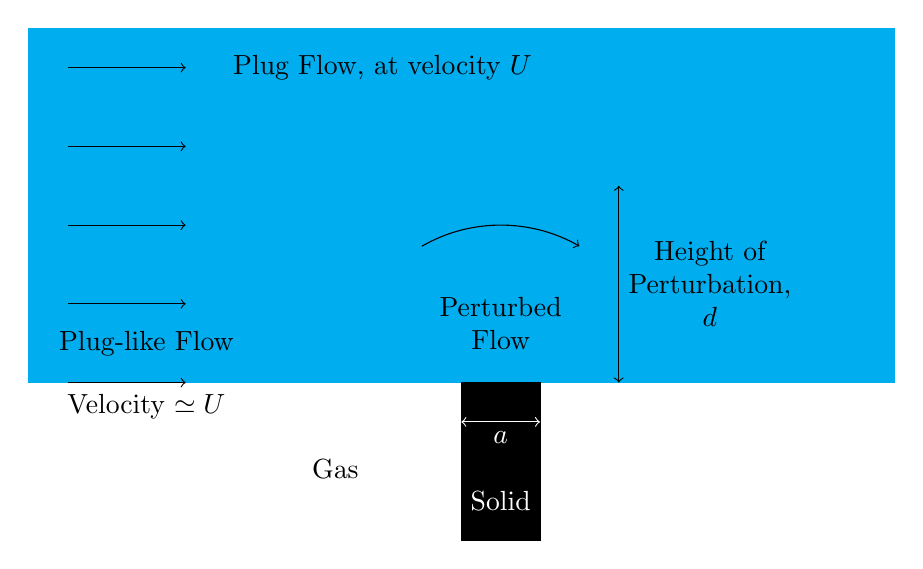
\begin{tikzpicture}

\filldraw[color=cyan] (-5.5,0) rectangle (5.5,4.5);
\filldraw (0,0) rectangle (1,-2);

\node at (-1.6,-1.1) {Gas};

\draw[<->,color=white] (0,-0.5) -- node [below] {$a$} ++(1,0);
\node at (0.5,-1.5) [color=white] {Solid};

\node at (0.5,0.75) [align=center] {Perturbed\\Flow};
\draw[<->] (2,0) -- node[right,align=center] {Height of \\Perturbation,\\ $d$} ++(0,2.5);

\draw (0.5,2) arc (90:120:2cm);
\draw[->] (0.5,2) arc (90:60: 2cm);

\foreach \z in {0,1,2,3,4}
     { \draw[->] (-5,\z) -- ++(1.5,0);
      % \draw[->] (4,\z) -- ++(1,0);
      }
       
\node at (-4,0.5) {Plug-like Flow};
\node at (-4,-0.3) {Velocity $\simeq U$};
%\node at (4,0.5)  {Plug-like Flow};
\node at (-1,4) {Plug Flow, at velocity $U$};
       
\end{tikzpicture}
\end{center}

The flow is mostly plug-like, with some characteristic velocity $U$.  The only place it is not plug-like is in the vicinity of the post.  The fluid sticks to the top of the post (no-slip), perturbing the plug-like flow.  The perturbed region extends some (arbitrary) distance $d$ above the post, at which point the velocity is (arbitrarily) close to $U$ again.  

\begin{center}
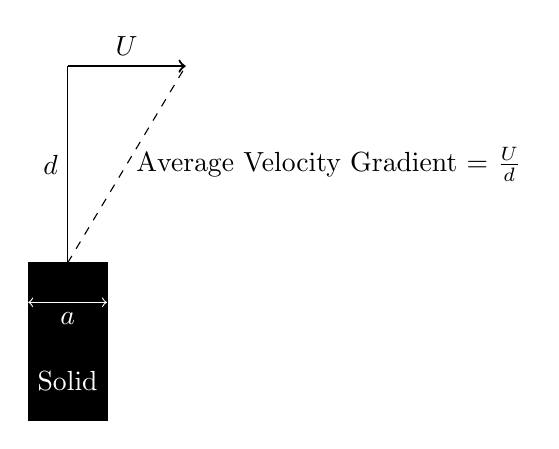
\begin{tikzpicture}

\filldraw (-0.5,0) rectangle ++(1,-2);
\draw[<->,color=white] (-0.5,-0.5) -- node [below] {$a$} ++(1,0);
\node at (0,-1.5) [color=white] {Solid};

\draw (0,0) -- node [left] {$d$} +(0,2.5);
\draw [->,thick] (0,2.5) -- node[above] {$U$} +(1.5,0);
\draw [dashed] (0,0) -- node[right] {Average Velocity Gradient = $\frac{U}{d}$} (1.5,2.5);

\end{tikzpicture}
\end{center}

Thus, the velocity changes from 0 to $U$ in distance $d$; the average velocity gradient is therefore
\begin{equation*}
\left< \frac{\partial u}{\partial z} \right> = \frac{U}{d}
\end{equation*}

Now, $d$ scales as $a$.  This is shown by dimensional analysis using the Buckingham Pi theorem in Appendix C.

Hence,
\begin{equation*}
\left< \frac{\partial u}{\partial z} \right> \sim \frac{U}{a}
\end{equation*}

Ybert and company justify the foregoing succintly: ``To estimate $ \left< \gamsol \right> $, we recall that the Stokes equation has a Laplacian form, which strongly couples the spatial dependence of the velocity profile along the different axes ($x,y,z$). This implies that $ \left< \gamsol \right> = \left< \partial u / \partial z \right> \sim U/a $, with $a$ the typical size of the solid area."

Thus, 
\begin{equation*}
\left< \sigsol \right> \sim \eta \frac{U}{a}
\end{equation*}
and
\begin{equation*}
\left< \sigma \right> \sim \phisol \eta \frac{U}{a}
\end{equation*}

The other interesting thing about mostly plug-like flow is that most of the fluid at the boundary is moving at the characteristic velocity $U$. So
\begin{equation*}
\left< u \right> \simeq U
\end{equation*}

Thus we have
\begin{equation*}
\eta \left< \dot{\gamma} \right> = \left< \sigma \right> \sim
  \frac{ \phisol \eta} {a} \left< u \right>
\end{equation*}
simplifying to:
\begin{equation*}
\left< u \right> \sim \frac{a}{\phisol}  \left< \dot{\gamma} \right>
\end{equation*}


defining
\begin{equation*}
\beff \sim  \frac{a}{\phisol} 
\end{equation*}

Thus in the limit of small solid fraction $\phisol$, Ybert \emph{et al} have shown that
\begin{equation*}
\beff \sim \alpha  \frac{a}{\phisol} 
\end{equation*}
where $\alpha$ is a prefactor that depends on the geometry of the surface.  This is the main result of Ybert \emph{et al} 2007 \cite{Ybert2007}.


\vspace{1em}
\colorbox[gray]{0.8}{ \textsc{Other Results} }
\vspace{0.5em}


Ybert \emph{et al} compare this scaling law with the exact result of J.\ R.\ Philip \cite{Philip1972}.  For the striped surface in question, $\phisol = a/L$, so the scaling law is:
\begin{equation*}
\beff \sim L
\end{equation*}
They note that in the limit of small $\phisol$, Philip's exact solution is similar, having only logarithmic dependence on $\phisol$: $\beff \sim L \log \phisol $


\vspace{1em}

If the surface is a forest of nanopillars, $\phisol = (a/L)^2$, so the scaling law is:
\begin{equation*}
\beff \sim  \frac{a}{\sqrt{ \phisol}} 
\end{equation*}

\vspace{1em}
Finally, if the no-slip condition is relaxed and some finite slip length $b_s$ holds on the solid post, the scaling law is modified to:
\begin{equation*}
\beff \sim  \frac{a + b_s}{\phisol} 
\end{equation*}

\vspace{1em}
For completeness, they consider the case of vanishing gas area.  Flow over a surface with very narrow gas gaps of width $l$ will be close to Couette flow, with:
\begin{equation*}
\beff \sim l (1-\phisol) 
\end{equation*}

The paper also features a few more formulae of a more speculative nature, which we won't mention here.

\subsection*{Numerics}

\paper{Ng \& Wang 2009}
As already mentioned, Ng and Wang in 2009 \cite{NgWang2009} did numerical studies of flow over a grating, in both parallel and transverse orientations. They derive eigenfunction expansions of the flow solutions, which are solved numerically.  The effective slip lengths extracted have essentially perfect agreement with the continuum modeling of Cottin-Bizonne 2004 \cite{Cottin-Bizonne2004}.

\sep

\paper{Davis \& Lauga 2009b}
In their second paper of 2009 \cite{DavisLauga2009b}, Davis and Lauga consider Stokes flow over a mesh of thin wires or strips, with large square air gaps in between.  The surface is considered to be flat, with no-slip on the strips, and perfect-slip on the liquid-air interface.  The period of the square-periodic mesh is $L$, and the width of the strips is $\epsilon L$.

\begin{center}
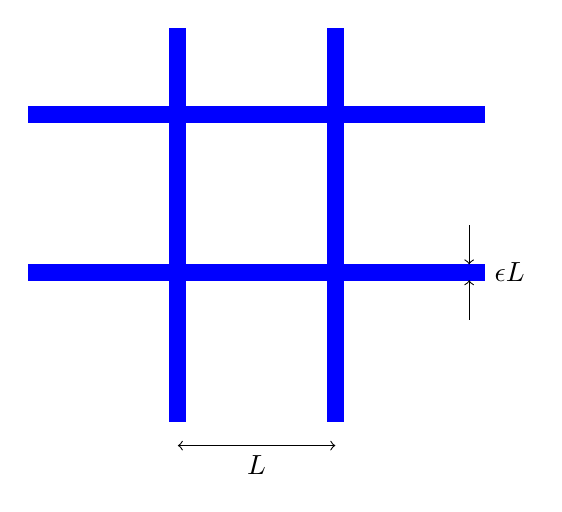
\begin{tikzpicture}

\filldraw[color=blue] (0,0) rectangle +(0.2,5);
\filldraw[color=blue] (2,0) rectangle +(0.2,5);
\draw[<->] (0.1,-0.3) -- node[below]{$L$} +(2,0);

\filldraw[color=blue] (-1.8,2) rectangle +(5.8,-0.2);
\filldraw[color=blue] (-1.8,4) rectangle +(5.8,-0.2);
\draw[<-] (3.8,2) -- +(0,0.5);
\draw[<-] (3.8,1.8) -- +(0,-0.5);
\node at (4,1.9)[right] {$\epsilon L$};

\end{tikzpicture}
\end{center}

Davis and Lauga use a method of superposition of singularities, and end up with an infinite system of linear equations.  Then $\beff = L/\pi (A_0 + B_0)$ where $A_0$ and $B_0$ are the zeroth-order coefficients of the system of equations.

They solve numerically for $A_0$ and $B_0$ by truncating the infinite system at $N$ equations.  (Truncating at $N=1000$ rather than $N=100$ changed the computed $\beff$ by less than $0.01\%$.) After computing $\beff$ for various values of $\epsilon$, they derive a least-squares fit formula:

\begin{equation*}
\beff = -0.107 L \ln \phisol + 0.003L
\end{equation*}

Finally, they offer `simple estimates' -- solutions from truncating the infinite series at $N=1$ and $N=2$ terms. For $N=1$:

\begin{equation*}
\beff = \frac{L}{3\pi} \ln \left( \frac{2}{\pi \epsilon} \right)
\end{equation*}

The simple estimate for $N=2$ is more complicated.  These simple estimates overestimate $\beff$ by up to 10\%, but converge on the correct result as $\epsilon \rightarrow 0$.

\subsection*{Coefficients Evaluated for Ybert's Scaling Laws}

The influential scaling law paper by Ybert \emph{et al} \cite{Ybert2007} inspired researchers to find the relevant coefficients by numerical or approximate methods.

\paper{Ng \& Wang 2010}
In 2010, Ng and Wang \cite{NgWang2010} continued their approach of numerically solving eigenfunction expansions, to find the scaling coefficients.

For flow over superhydrophobic surfaces, with the solid posts occupying a small area fraction, Ybert had proposed:
\begin{equation*}
\beff \sim \frac{1}{\sqrt{\phisol}}
\end{equation*}
From their numerical data, Ng and Wang fit the parameters:

\begin{align*}
\beff &= \frac{0.34}{\sqrt{\phisol}} - 0.468 \quad \text{for circular posts,} \\
\beff &= \frac{0.33}{\sqrt{\phisol}} - 0.461 \quad \text{for square posts.}
\end{align*}

And so on and so on.  Ng and Wang present numerically fitted parameters for the nanobubble case ($\phisol \rightarrow 1$), for cases with finite slip on the solid, and for cases where the geometry is elliptical or rectangular rather than simply circular or square.

\sep

\paper{Davis \& Lauga 2010}
In 2010, Davis and Lauga \cite{DavisLauga2010} studied Stokes flow over a superhydrophobic surface comprising a rectangular array of circular posts, each of radius $a$.

\begin{center}
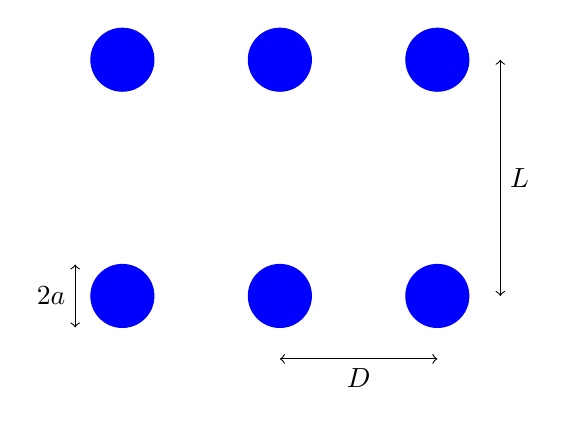
\begin{tikzpicture}

\filldraw[color=blue] (0,0) circle (4mm);
\filldraw[color=blue] (2,0) circle (4mm);
\filldraw[color=blue] (4,0) circle (4mm);
\filldraw[color=blue] (0,3) circle (4mm);
\filldraw[color=blue] (2,3) circle (4mm);
\filldraw[color=blue] (4,3) circle (4mm);

\draw[<->] (-0.6,-0.4) -- node[left]{$2a$} +(0,0.8);
\draw[<->] (2,-0.8) -- node[below]{$D$} +(2,0);
\draw[<->] (4.8,0) -- node[right]{$L$} +(0,3);

\end{tikzpicture}
\end{center}

As their point of departure, they take the scaling law proposed in Ybert \emph{et al} 2007 for the limit of small $\phisol$:
\begin{equation*}
\beff \sim \frac{A}{\sqrt{\phisol}} L - BL
\end{equation*}

They attack the problem with Fourier transform techniques, and end up with an infinite system of linear equations for coefficients.  They make an `asymptotic estimate' of the coefficients, and get:
\begin{equation*}
\beff \sim \frac{3}{16} \sqrt{ \frac{\pi}{\phisol}} \sqrt{DL}
\end{equation*}
If the array is square, this reduces to:
\begin{equation*}
\beff \sim \frac{3}{16} \sqrt{ \frac{\pi}{\phisol}} L
\end{equation*}
Adding the next-order correction term gives (for the square array):
\begin{equation*}
\beff \sim \frac{3}{16} \sqrt{ \frac{\pi}{\phisol}} L - \frac{3}{2\pi} \ln(1 + \sqrt{2})L
\end{equation*}
in the limit of low $\phisol$.

They compare their analytical asymptotic estimate with previous numerical work: ``The quantitative agreement between our model and previous numerical work is remarkable... we find that the error between our simple model, and numerics of Ng and Wang (2010) \cite{NgWang2010} is about 1.8\%, while the error between our model and the computations of Ybert \emph{et al} (2007) \cite{Ybert2007} is about 3.9\%."



\section*{Conclusion}

There exists only on the order of a dozen expressions for the effective slip length of a mixed-slip surface.  Only a handful of them are exact results that have been rigorously derived, including the seminal work of J.\ R.\ Philip in 1972 \cite{Philip1972}, the work of Lauga and Stone in 2003 \cite{LaugaStone2003}, and our own recent papers \cite{HendyLund2007,LundHendy2008,Lund2012}, which form the core of this thesis.

A simple phenomenological model was proposed by the Lyon group in the paper by Cottin-Bizonne \emph{et al} \cite{Cottin-Bizonne2004}, leading to the suggestion that
\begin{equation*}
\beff = \left<  \frac{1}{b} \right>^{-1}
\end{equation*}
This thesis proves this and extends it to the case of rough surfaces.  The same model inspired the derivation of several scaling laws, which appear in the highly influential paper of 2007 by Ybert \emph{et al} \cite{Ybert2007}.

The scaling laws have been refined by various researchers, by finding appropriate coefficients via numerical or approximate methods.

\begin{center} \vspace{3em} \Coffeecup \end{center}

\bibliography{Lund_Thesis.bib}
\bibliographystyle{plain}

\end{document}
